\documentclass[handout]{beamer}

\usetheme[progressbar=frametitle]{metropolis}
\usepackage{appendixnumberbeamer}
\usepackage{booktabs}
\usepackage{amsmath}
\usepackage{amssymb}
\usepackage{tcolorbox}
\definecolor{metropolisblue}{RGB}{39, 59, 94}
\usepackage{xcolor}

% Define custom colors
\definecolor{myblue}{HTML}{007AFF}
\definecolor{mygreen}{HTML}{4CD964}
\definecolor{myred}{HTML}{FF3B30}
\definecolor{myorange}{HTML}{FF9500}



% Begin document
\begin{document}

% Title page
\title{Introduction}
\author{Nipun Batra}
\date{\today}
\institute{IIT Gandhinagar}
\maketitle

\begin{frame}{What}
    \begin{itemize}
        \item Predict with uncertainty
        \item Optimize any black box function
        \item Efficiently create a training set
        \item Generative modelling
    \end{itemize}

    
\end{frame}

\begin{frame}{Dog or Cat?}  
    
\end{frame}

\begin{frame}{Far from the Moon}
    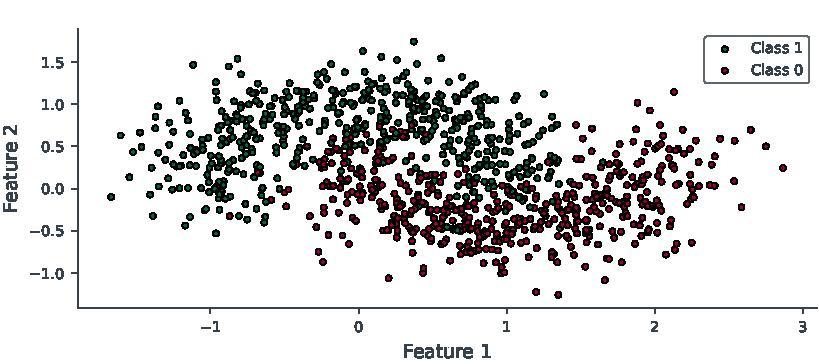
\includegraphics[width=\textwidth]{../figures/introduction/gp_classification_data.pdf}    

    
\end{frame}

\begin{frame}{Far from the Moon}
    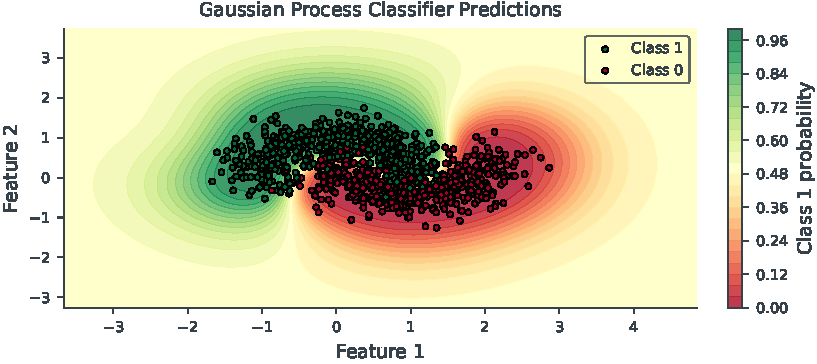
\includegraphics[width=\textwidth]{../figures/introduction/gp_classification-3.pdf}    

    
\end{frame}

\begin{frame}{Global Warming?}
    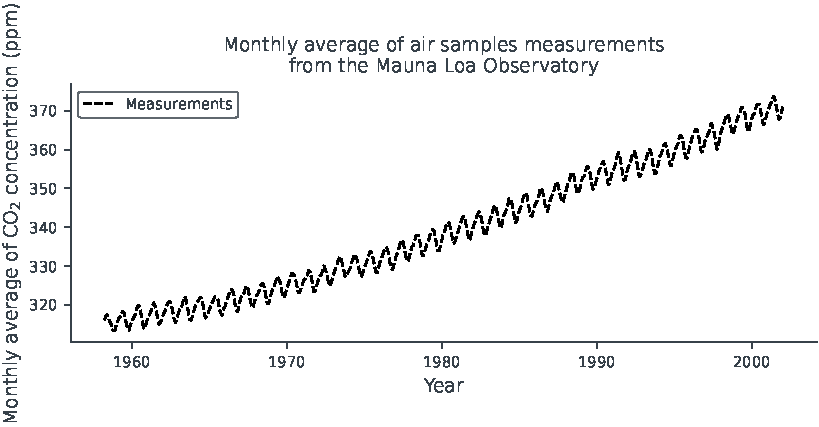
\includegraphics[width=\textwidth]{../figures/introduction/co2_data.pdf}    
    
\end{frame}

\begin{frame}{Global Warming?}
    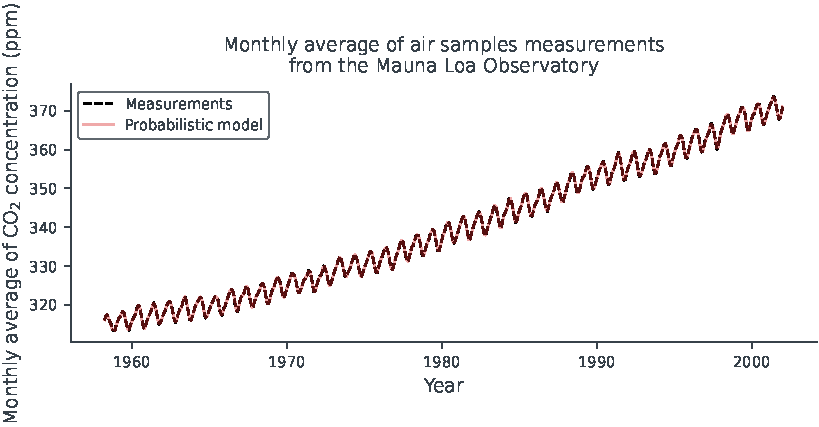
\includegraphics[width=\textwidth]{../figures/introduction/train_fit.pdf}    
    
\end{frame}

\begin{frame}{Global Warming?}
    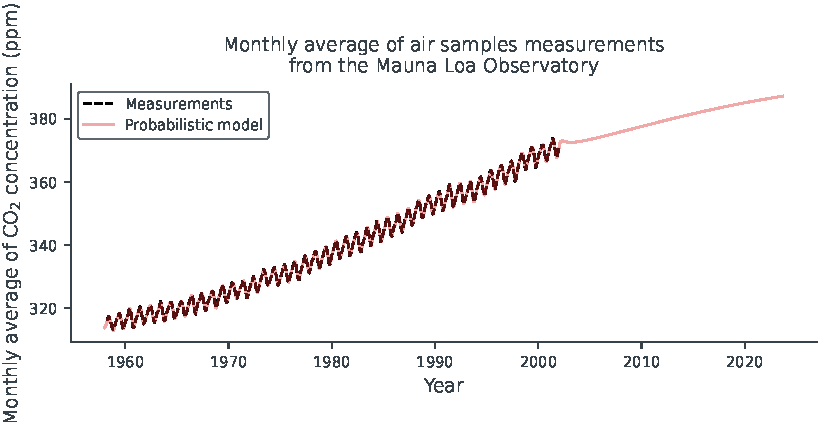
\includegraphics[width=\textwidth]{../figures/introduction/future_mean.pdf}    
    
\end{frame}

\begin{frame}{Global Warming?}
    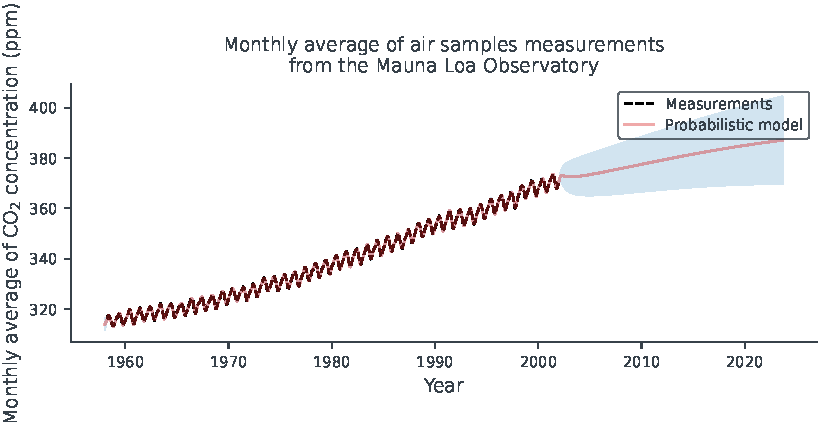
\includegraphics[width=\textwidth]{../figures/introduction/future_full.pdf}    
    
\end{frame}

\begin{frame}{Identify the person}
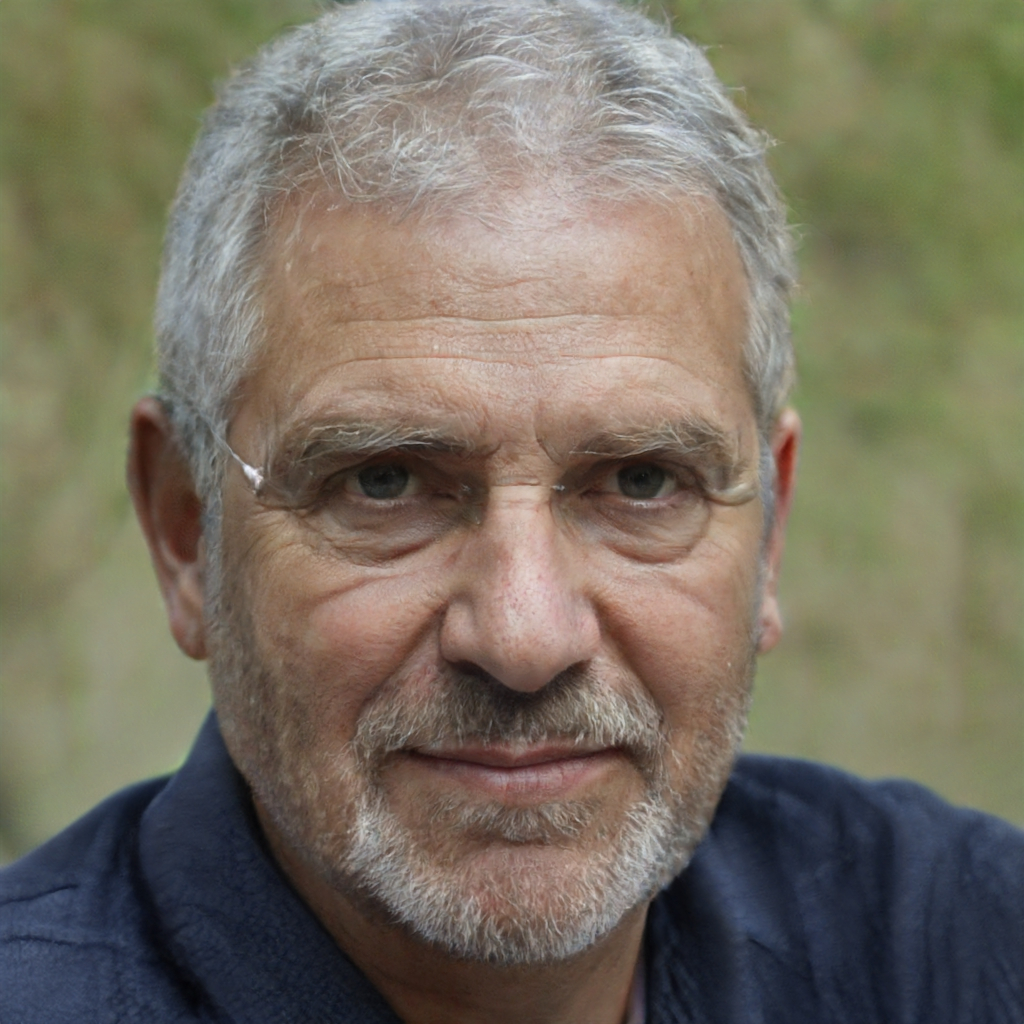
\includegraphics[height=\textwidth]{../figures/introduction/famous.jpeg}    
\end{frame}

\begin{frame}{Identify the person}
    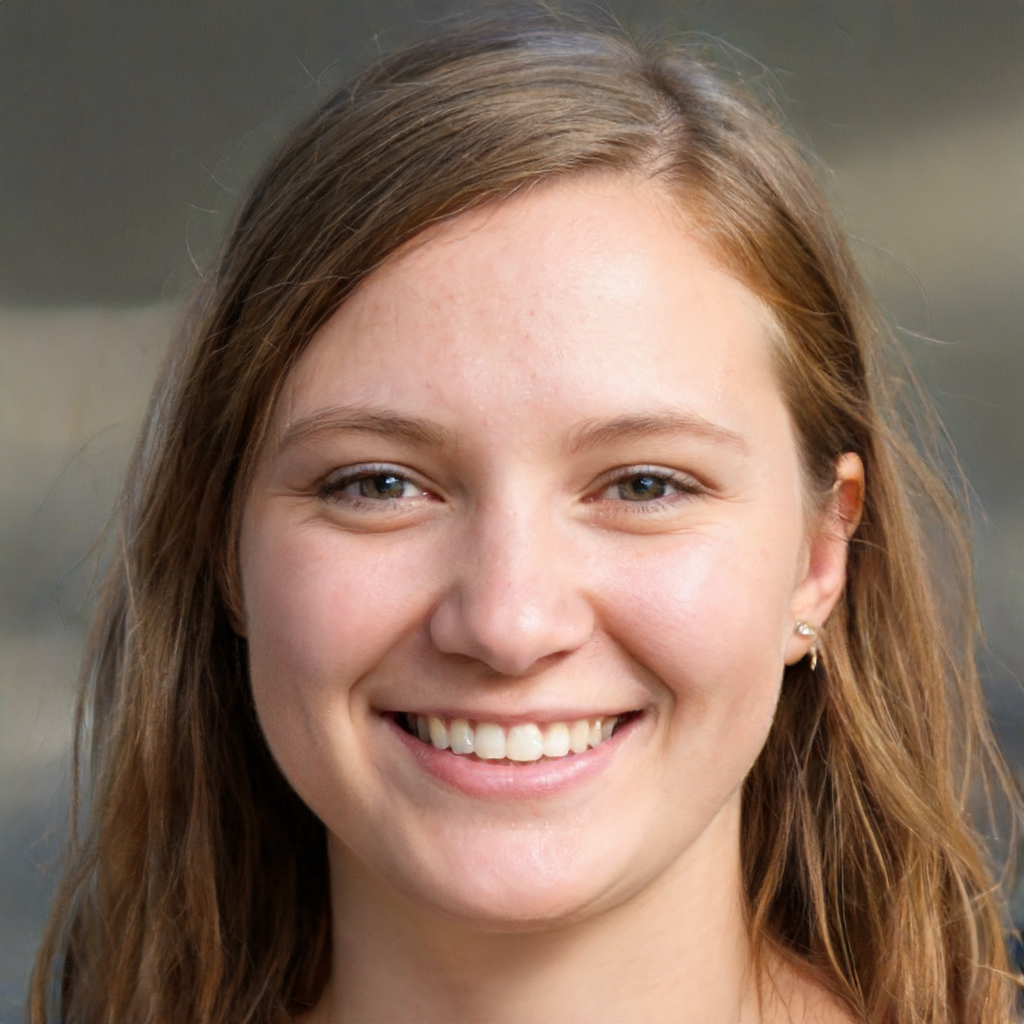
\includegraphics[height=\textwidth]{../figures/introduction/famous-2.jpeg}    
    \end{frame}


\begin{frame}{Questions}
    \begin{itemize}
        \item We used squared error loss function for linear regression. Why?
        \item We used cross entropy loss function for logistic regression. Why?
        \item How does np.random.randn work?
        \item np.std(x) and pd.std(x) give different results. Why?

    \end{itemize}
    
\end{frame}

\begin{frame}{Quiz time}
    \href{https://www.3blue1brown.com/lessons/bayes-theorem}{Farmer or Librarian? (3Blue1Brown)} 
\end{frame}

\begin{frame}{Bayes Rule}
    \begin{equation*}
        P(A|B) = \frac{P(B|A)P(A)}{P(B)}
    \end{equation*}
    
    Rewriting it using the ML notation:
    \begin{equation*}
        \textcolor{myblue}{P(\theta|D)} = \frac{\textcolor{mygreen}{P(D|\theta)} \cdot \textcolor{myred}{P(\theta)}}{\textcolor{myorange}{P(D)}}
    \end{equation*}
    
    \begin{itemize}
        \item \textcolor{myblue}{$P(\theta|D)$} is called the posterior
        \item \textcolor{mygreen}{$P(D|\theta)$} is called the likelihood
        \item \textcolor{myred}{$P(\theta)$} is called the prior
        \item \textcolor{myorange}{$P(D)$} is called the evidence
    \end{itemize}
\end{frame}



\begin{frame}{One Equation Throughout the Course}
    \begin{equation*}
        \textcolor{myblue}{P(\theta|D)} = \frac{\textcolor{mygreen}{P(D|\theta)} \cdot \textcolor{myred}{P(\theta)}}{\textcolor{myorange}{P(D)}} = \frac{\textcolor{mygreen}{P(D|\theta)} \cdot \textcolor{myred}{P(\theta)}}{\int_{\theta} \textcolor{mygreen}{P(D|\theta)} \cdot \textcolor{myred}{P(\theta)} d\theta}
    \end{equation*}

    %tcolorbox
    \begin{tcolorbox}[colback=metropolisblue!5,colframe=metropolisblue,title=I. Maximum Likelihood Estimation]
        Given a dataset $D$, find the parameters $\theta$ that maximize the likelihood of the data.
        \begin{equation*}
            \theta_{\text{MLE}} = \arg \max_{\theta} \textcolor{mygreen}{P(D|\theta)}
        \end{equation*}
    For example, given a linear regression problem setup, we set the likelihood as normal distribution and find the parameters $\theta$ that maximize the likelihood of the data.
    \end{tcolorbox}
        
    
\end{frame}


\begin{frame}{One Equation Throughout the Course}
    \begin{equation*}
        \textcolor{myblue}{P(\theta|D)} = \frac{\textcolor{mygreen}{P(D|\theta)} \cdot \textcolor{myred}{P(\theta)}}{\textcolor{myorange}{P(D)}} = \frac{\textcolor{mygreen}{P(D|\theta)} \cdot \textcolor{myred}{P(\theta)}}{\int_{\theta} \textcolor{mygreen}{P(D|\theta)} \cdot \textcolor{myred}{P(\theta)} d\theta}
    \end{equation*}

    %tcolorbox
    \begin{tcolorbox}[colback=metropolisblue!5,colframe=metropolisblue,title=II. Maximum A Posteriori Estimation]
        Given a dataset $D$, find the parameters $\theta$ that maximize the posterior of the data considering both the likelihood and the prior.
        \begin{equation*}
            \theta_{\text{MAP}} = \arg \max_{\theta} \textcolor{myblue}{P(\theta|D)} = \arg \max_{\theta} \textcolor{mygreen}{P(D|\theta)} \cdot \textcolor{myred}{P(\theta)}
        \end{equation*}

    For example, given a linear regression problem, we assume prior over the parameters $\theta$ and find the parameters $\theta$ that maximize the posterior of the data.
    \end{tcolorbox}
        
    
\end{frame}


\begin{frame}{One Equation Throughout the Course}
    \begin{equation*}
        \textcolor{myblue}{P(\theta|D)} = \frac{\textcolor{mygreen}{P(D|\theta)} \cdot \textcolor{myred}{P(\theta)}}{\textcolor{myorange}{P(D)}} = \frac{\textcolor{mygreen}{P(D|\theta)} \cdot \textcolor{myred}{P(\theta)}}{\int_{\theta} \textcolor{mygreen}{P(D|\theta)} \cdot \textcolor{myred}{P(\theta)} d\theta}
    \end{equation*}


    %tcolorbox
    \begin{tcolorbox}[colback=metropolisblue!5,colframe=metropolisblue,title=III. Bayesian Inference with Conjugate Priors]
       Find full posterior: $P(\theta|D)$ given likelihood $P(D|\theta)$ and prior $P(\theta)$ where the prior and the posterior belong to the same family of distributions.

 
    \end{tcolorbox}
 
    
\end{frame}

\begin{frame}{One Equation Throughout the Course}
    \begin{equation*}
        \textcolor{myblue}{P(\theta|D)} = \frac{\textcolor{mygreen}{P(D|\theta)} \cdot \textcolor{myred}{P(\theta)}}{\textcolor{myorange}{P(D)}} = \frac{\textcolor{mygreen}{P(D|\theta)} \cdot \textcolor{myred}{P(\theta)}}{\int_{\theta} \textcolor{mygreen}{P(D|\theta)} \cdot \textcolor{myred}{P(\theta)} d\theta}
    \end{equation*}


    %tcolorbox
    \begin{tcolorbox}[colback=metropolisblue!5,colframe=metropolisblue,title=IV. Main Challenge in Bayesian Inference]
        Compute the evidence $P(D)$ is intractable in most cases. It involves integrating over all possible values of $\theta$. Thus, computing the posterior $P(\theta|D)$ is intractable in most cases.
 
    \end{tcolorbox}
 
    
\end{frame}

\begin{frame}{One Equation Throughout the Course}
    \begin{equation*}
        \textcolor{myblue}{P(\theta|D)} = \frac{\textcolor{mygreen}{P(D|\theta)} \cdot \textcolor{myred}{P(\theta)}}{\textcolor{myorange}{P(D)}} = \frac{\textcolor{mygreen}{P(D|\theta)} \cdot \textcolor{myred}{P(\theta)}}{\int_{\theta} \textcolor{mygreen}{P(D|\theta)} \cdot \textcolor{myred}{P(\theta)} d\theta}
    \end{equation*}


    %tcolorbox
    \begin{tcolorbox}[colback=metropolisblue!5,colframe=metropolisblue,title=Va. Approx. Bayesian Inference with Variational Inference]
        Approximate the posterior $P(\theta|D)$ with a tractable distribution $Q_\phi (\theta)$ characterized by a set of parameters $\phi$.
        Our goal is to find the parameters $\phi$ that minimize the KL divergence between the approximate posterior $Q_\phi (\theta)$ and the true posterior $P(\theta|D)$.

        \begin{equation*}
            \phi_{\text{VI}} = \arg \min_{\phi} \textcolor{myblue}{\text{KL}} \left( Q_\phi (\theta) || P(\theta|D) \right)
        \end{equation*}
 
    \end{tcolorbox}
 
    
\end{frame}

\begin{frame}{One Equation Throughout the Course}
    \begin{equation*}
        \textcolor{myblue}{P(\theta|D)} = \frac{\textcolor{mygreen}{P(D|\theta)} \cdot \textcolor{myred}{P(\theta)}}{\textcolor{myorange}{P(D)}} = \frac{\textcolor{mygreen}{P(D|\theta)} \cdot \textcolor{myred}{P(\theta)}}{\int_{\theta} \textcolor{mygreen}{P(D|\theta)} \cdot \textcolor{myred}{P(\theta)} d\theta}
    \end{equation*}


    %tcolorbox
    \begin{tcolorbox}[colback=metropolisblue!5,colframe=metropolisblue,title=Vb. Approx. Bayesian Inference with Laplace Approximation]
        Approximate the posterior $P(\theta|D)$ with a Gaussian distribution centered at the MAP estimate $\theta_{\text{MAP}}$ and the covariance matrix is the inverse of the Hessian matrix of the negative log posterior evaluated at $\theta_{\text{MAP}}$.
 
        \begin{equation*}
            P(\theta|D) \approx \mathcal{N} \left( \theta | \theta_{\text{MAP}}, H^{-1} \right)
        \end{equation*}
        \begin{equation*}
            H = - \nabla^2 \log P(\theta|D) \bigg|_{\theta = \theta_{\text{MAP}}}
        \end{equation*}

    \end{tcolorbox}
 
    
\end{frame}




\begin{frame}{One Equation Throughout the Course}
    \begin{equation*}
        \textcolor{myblue}{P(\theta|D)} = \frac{\textcolor{mygreen}{P(D|\theta)} \cdot \textcolor{myred}{P(\theta)}}{\textcolor{myorange}{P(D)}} = \frac{\textcolor{mygreen}{P(D|\theta)} \cdot \textcolor{myred}{P(\theta)}}{\int_{\theta} \textcolor{mygreen}{P(D|\theta)} \cdot \textcolor{myred}{P(\theta)} d\theta}
    \end{equation*}


    %tcolorbox
    \begin{tcolorbox}[colback=metropolisblue!5,colframe=metropolisblue,title=Vc. Approx. Bayesian Inference with Sampling Methods]
        It is intractable to compute the posterior $P(\theta|D)$ in most cases. But, we can instead get samples from the posterior $P(\theta|D)$. 
 
    \end{tcolorbox}
 
    
\end{frame}

\begin{frame}{One Equation Throughout the Course}
    \begin{equation*}
        \textcolor{myblue}{P(\theta|D)} = \frac{\textcolor{mygreen}{P(D|\theta)} \cdot \textcolor{myred}{P(\theta)}}{\textcolor{myorange}{P(D)}} = \frac{\textcolor{mygreen}{P(D|\theta)} \cdot \textcolor{myred}{P(\theta)}}{\int_{\theta} \textcolor{mygreen}{P(D|\theta)} \cdot \textcolor{myred}{P(\theta)} d\theta}
    \end{equation*}




    %tcolorbox
    \begin{tcolorbox}[colback=metropolisblue!5,colframe=metropolisblue,title=VI. Approx. Integrals with Monte Carlo Integration]
       
    Aim: predict the model's output $y^*$ at a new input $x^*$. 

    \begin{equation*}
        P(y^*|x^*, D) = \int_{\theta} P(y^*|x^*, \theta) \cdot P(\theta|D) d\theta
    \end{equation*}
    We can instead use Monte Carlo integration to approximate the above integral as follows:
    \begin{equation*}
        P(y^*|x^*, D) \approx \frac{1}{S} \sum_{s=1}^S P(y^*|x^*, \theta_s)
    \end{equation*}
    where $\theta_s \sim P(\theta|D)$.
    \end{tcolorbox}
 
    
\end{frame}


    

\end{document}